\chapter{Návrh}
V tejto kapitole je uvedený návrh architektúry softwarovej aplikácie pomocou C4 modelu.
Nasleduje návrh štruktúry databázy, kde nájdeme aj schémy vytvárajúce tabuľky v databáze. 

Zároveň tu nájdeme aj návrh jednotlivých SPARQL dotazov, ktoré sú potrebne pre fungovanie aplikácie. 

\section{Návrh softvérovej architektúry}

Softwarovú architektúru vyjadríme pomocou C4 modelu. Model pomáha opísať softwarovú architektúru počas
návrhu samotnej architektúry a pri spätnom dokumentovaní už existujúceho kódu.

C4 model využíva prístup "abstrakcia na prvom mieste" k vytváraniu diagramov softwarovej architektúry, ktoré vznikli na základe
abstrakcie reprezentujúcej uvažovanie architekta nad softvérom.

Na začiatok je ale potrebné definovať spoločnú sadu abstrakcii na vytvorenie jazyka vhodného na opis statickej štruktúry softvérového systému.
Najvyššia úroveň abstrakcie je Softwarový systém. Ten opisuje prínosnú hodnotu používateľovi používajúci systém, či už je to človek alebo iný systém.
Softwarový systém je tvorení z jedného alebo viacerých kontajnerov. Kontajner v C4 modely reprezentujú aplikácie a dátové úložiská.
Pre funkčné fungovanie softvérového systém je potrebné aby kontajneri boli spustené, bežali.

Každý kontajner je tvorený jedným alebo viacerými komponentami, ktoré sú implementované jedným alebo viacerými kódovými elementami. Pojmom “kódový element” myslíme
triedy, objekty, funkcie a podobne. V kontexte C4 modelu je pojem “komponentom” myslené zoskupenie súvisiacich funkcii zapuzdrených za dobre definovaným rozhraním.
Softwerový system môžu využivať osoby, reprezentujúce jedného zo skupiný ľudi použivajucích softwerový systém.

Model pozostáva zo štyroch úrovní:
\begin{enumerate}
      \item Systém Kontext diagram - zobrazuje systém ako krabicu v strede, obklopenú osobami a inými systémami, ktoré interagujú so systémom.
            Detaily ako technológie, protokoly a iné low-level detaily na tejto úrovni nie sú dôležité. Dôraz kladieme na osoby a softwarový systém.
      \item Kontajner diagram - zobrazuje high-level tvar softvérovej architektúry, ako sú v nej rozdelené zodpovednosti. Zároveň zobrazuje technologické rozhodnutia a
            spôsob ako kontajneri medzi sebou komunikujú.
      \item Komponent diagram - zobrazuje z čoho pozostáva konkrétny kontajner, aké sú jeho komponenty, ich zodpovednosť a technologické detaily.
      \item Kód diagram - zobrazuje ako sú komponenty implementované kódom
\end{enumerate}

Pre vyjadrenie softvérovej architektúry nie je potrebne využiť všetky úrovne.
Často krát je postačujúce využiť iba Kontextovú a Kontajnerovú úroveň.

V nasledujúcich sekciách vyjadríme pomocou C4 modelu našu softwarovú architektúru v každej úrovni, okrem najnižšej úrovne Kód pomocou UML diagramov, ktoré nájdeme na obrázkoch.

zdroj : https://c4model.com/

\subsection{Systém Kontext diagram}

\begin{figure}[h]
      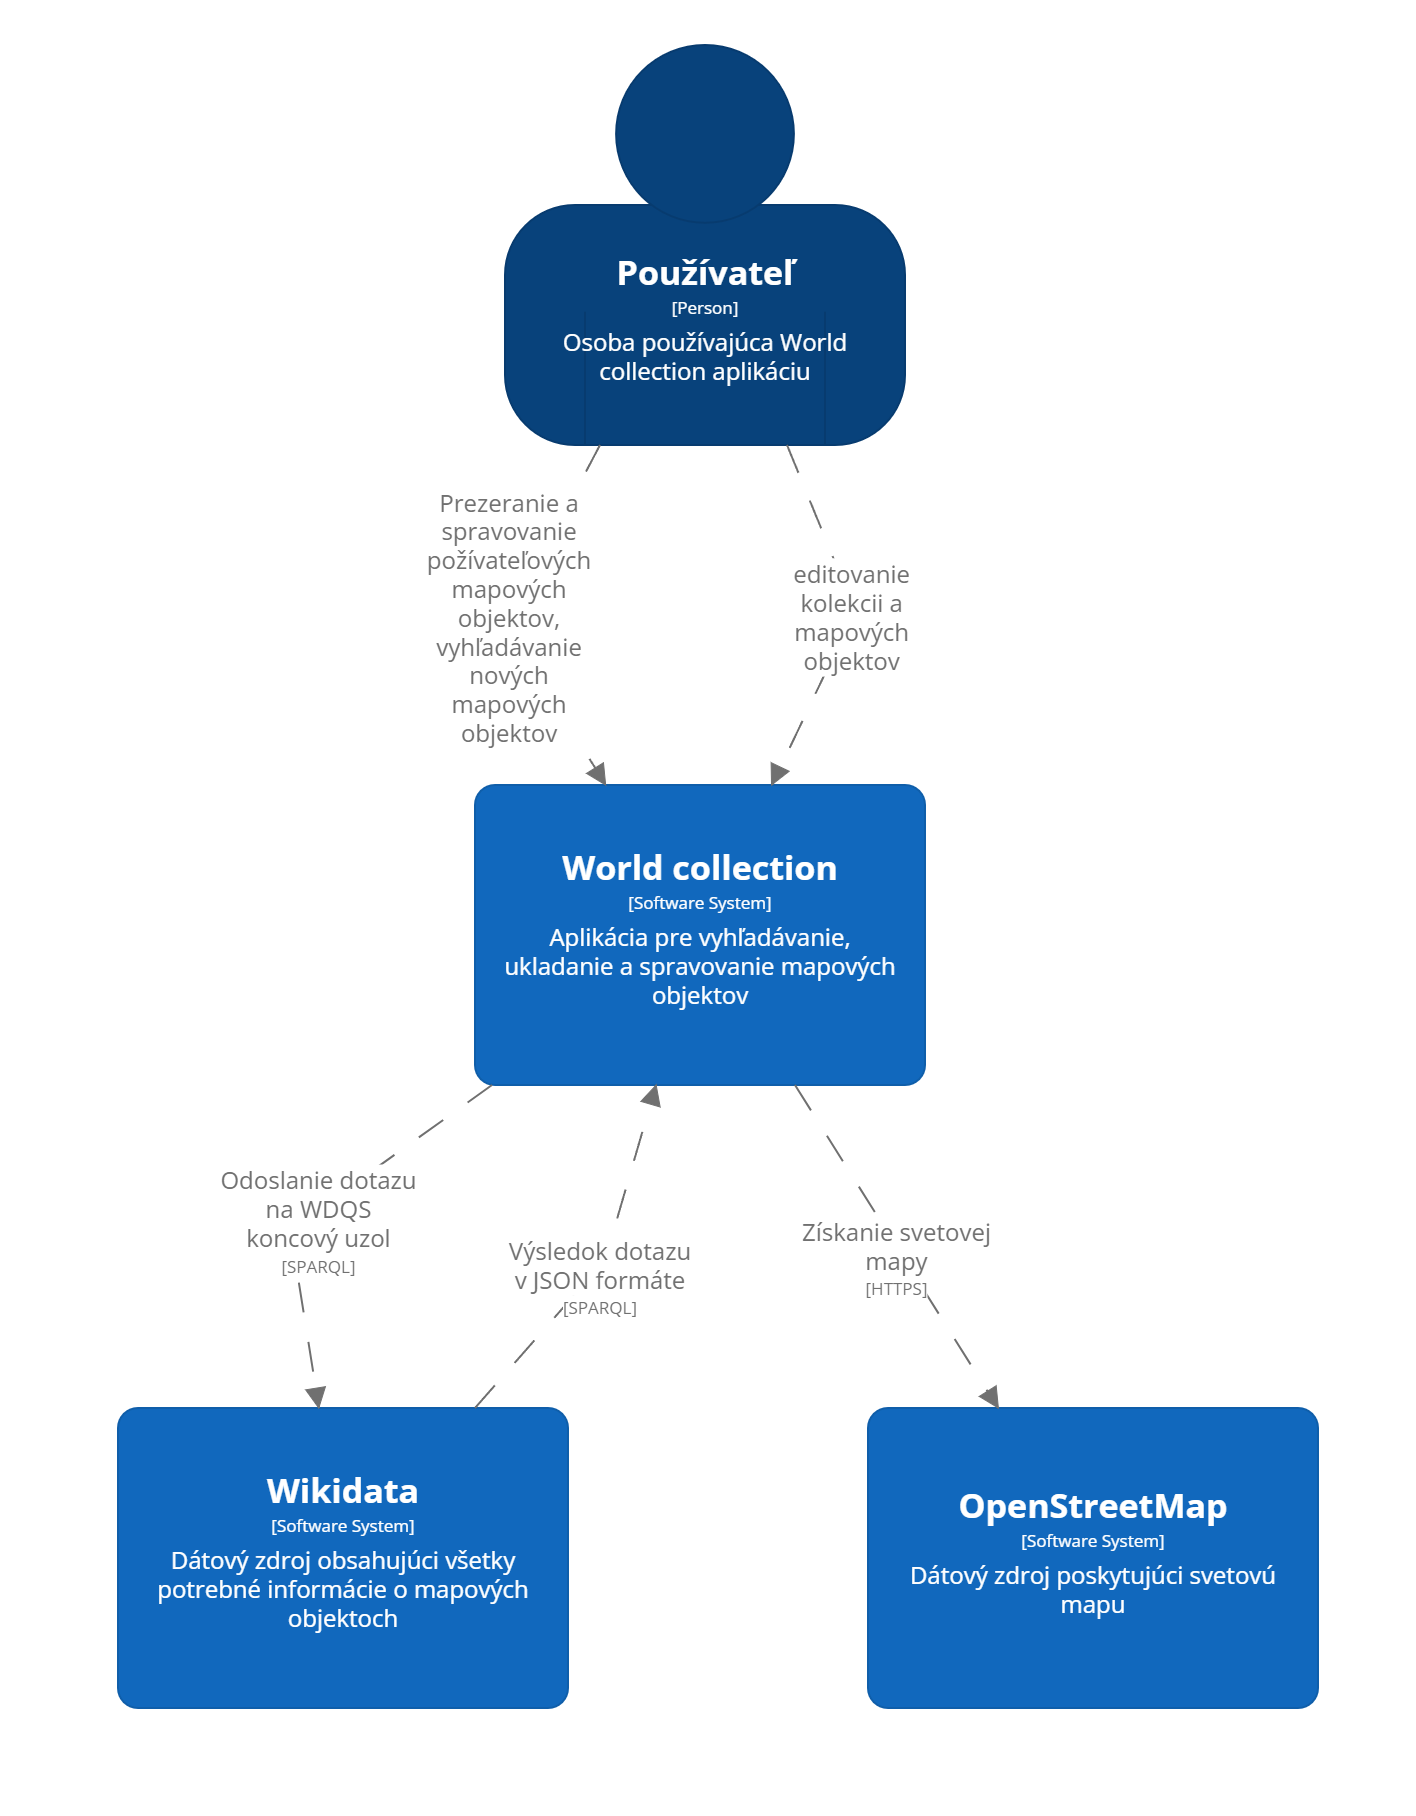
\includegraphics[width=140mm]{../img/structurizr-SystemContext}
      \caption{Systém Kontext diagram}
\end{figure}

V najvyššej úrovni abstrakcie je najdôležitejšia krabica v strede, ktorá reprezentuje náš softwarový systém “World collection”. Tento systém je používaný používateľom.
Používateľ je osoba využívajúca systém na vyhľadanie a spravovanie mapových objektov.
Okolo nášho systému sú aj iné systémy reprezentujúce dátové zdroje, s ktorými náš systém interaguje. Tieto systémy sú nevyhnutnou
súčasťou celej architektúry a bez nich by aplikácia nevedela fungovať.

Pre získanie svetovej mapy bude náš systém komunikovať s OpenStreetMap. Tie  poskytnú systému dáta svetovej mapy pre vytvorenie interaktívnej mapy sveta.

Všetky informácie a dáta ohľadom mapových objektov bude systém získavať z Wikidát.

\subsection{Kontajner diagram }

\begin{figure}[h]
      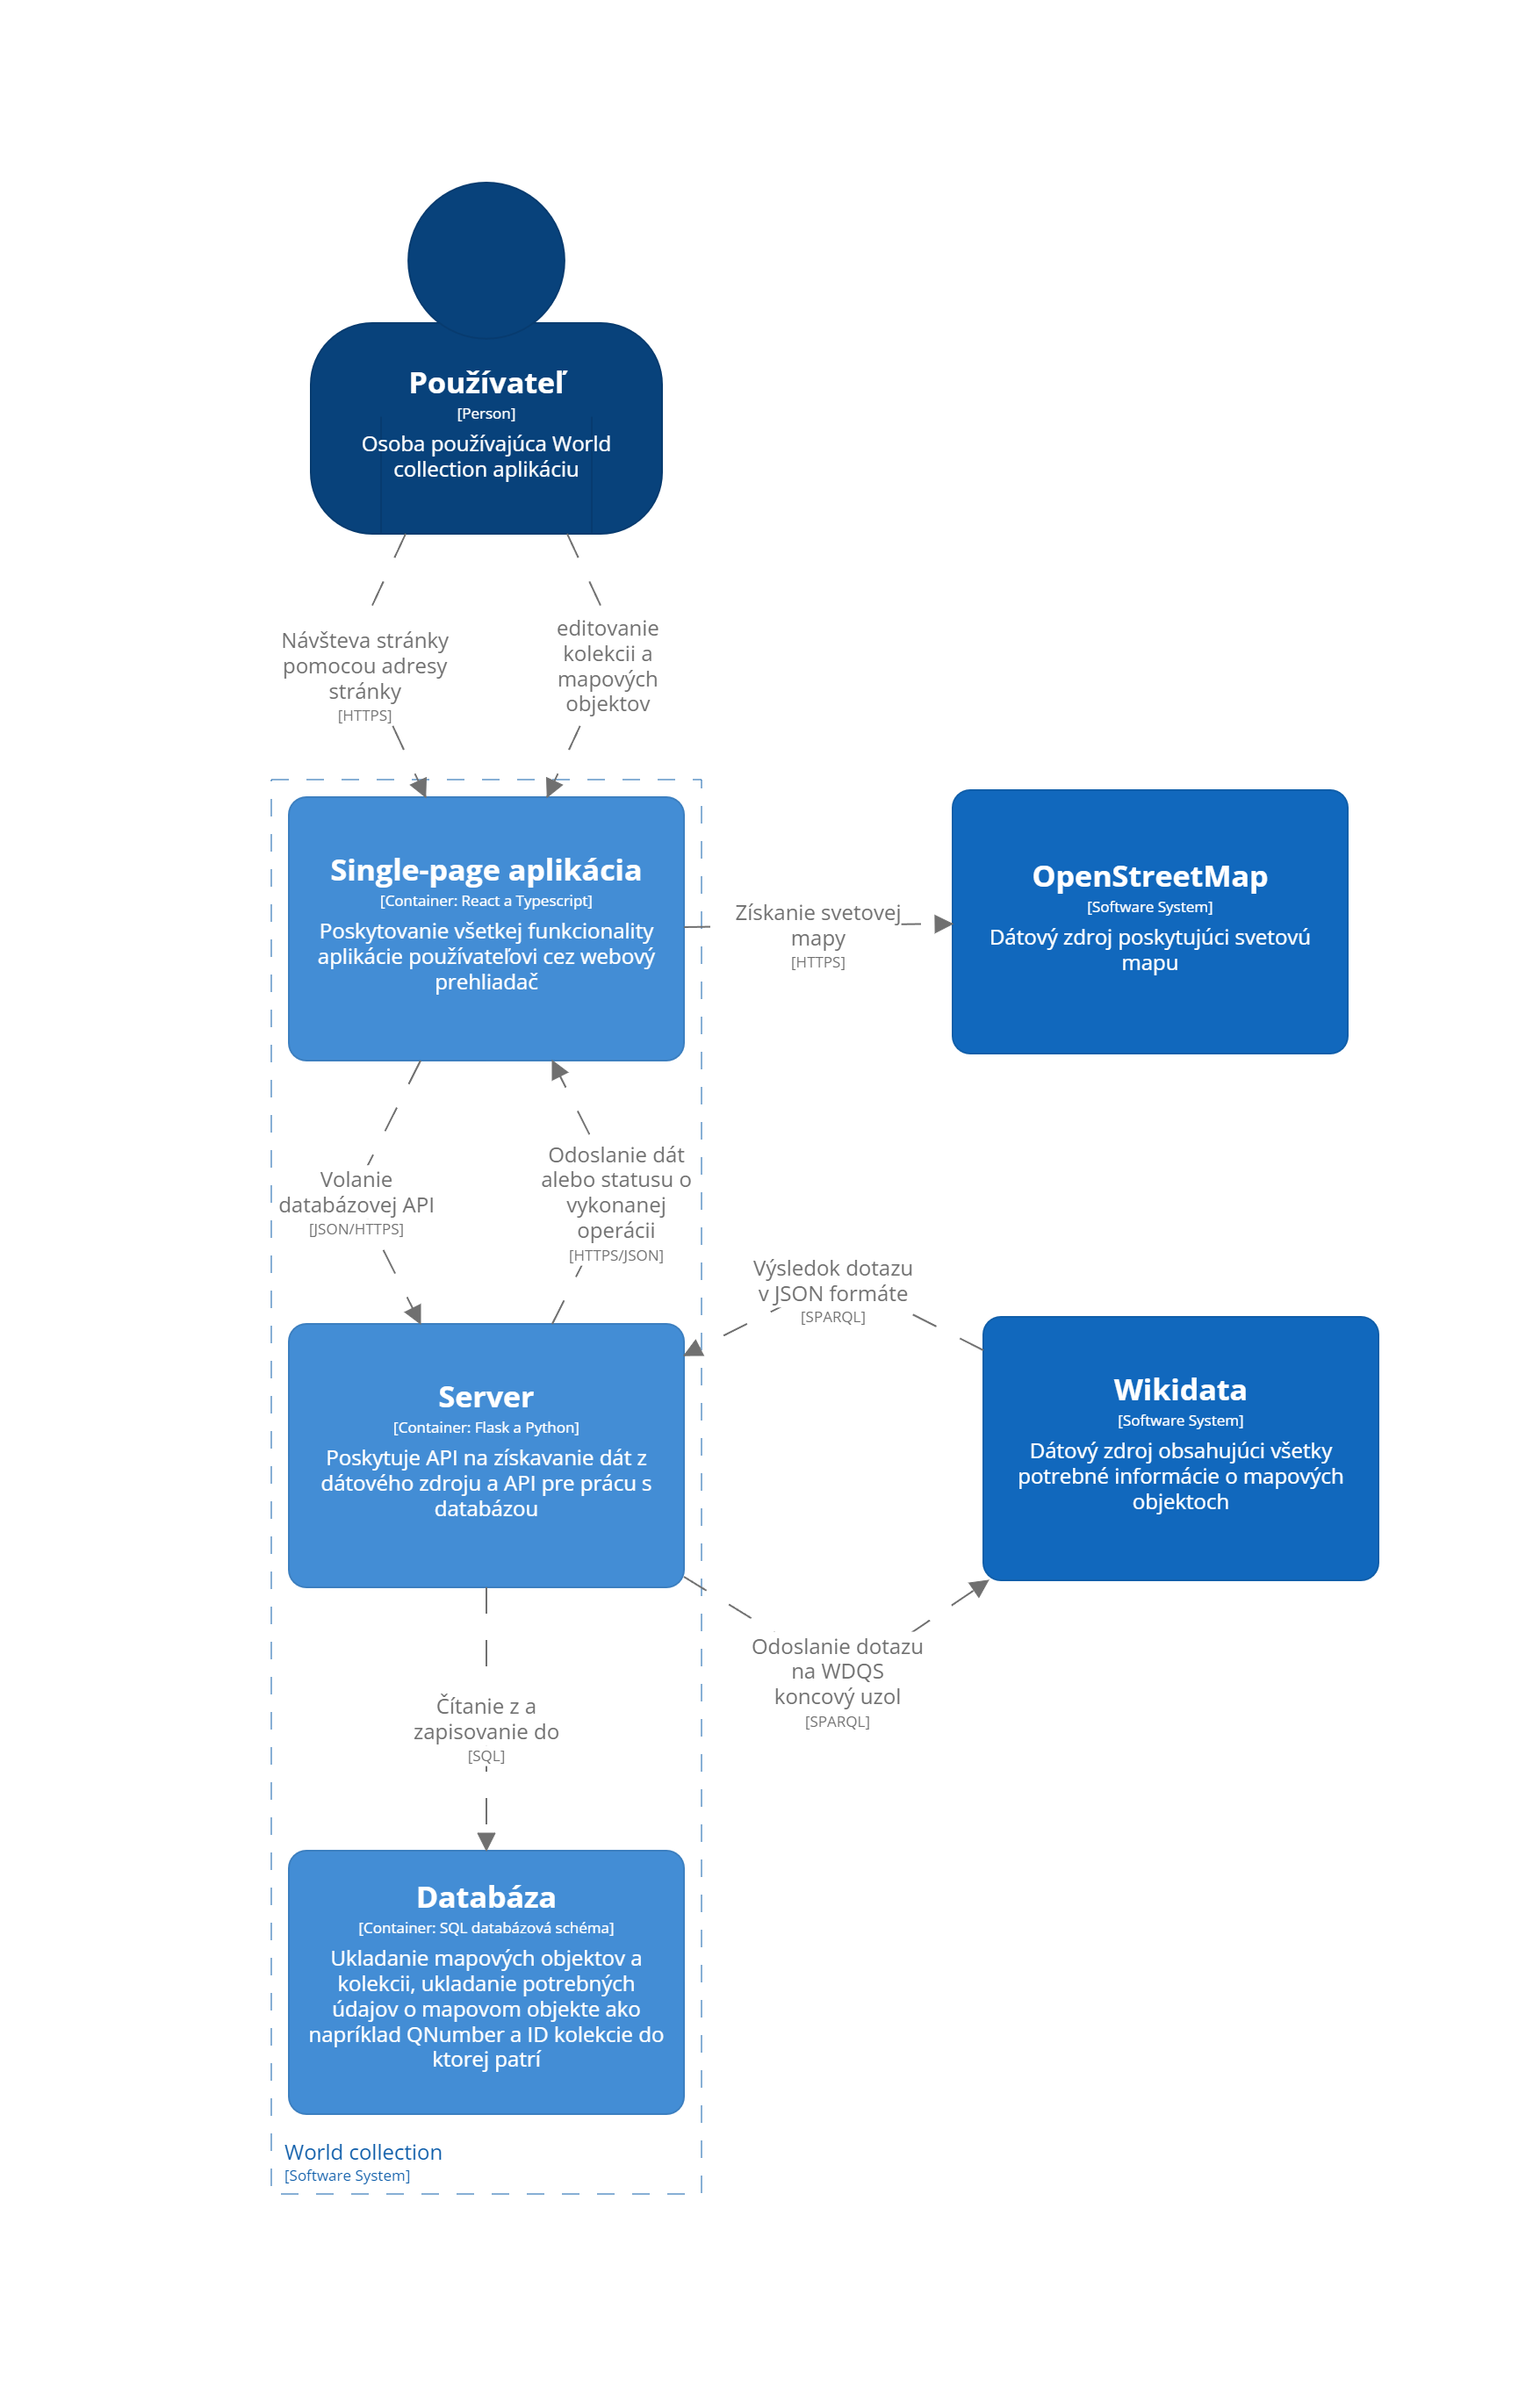
\includegraphics[width=140mm]{../img/structurizr-Containers}
      \caption{Kontajner diagram }
\end{figure}

World collection je single-page webová aplikácia. Z toho dôvodu aplikácia pozostáva z dvoch hlavných časti: backend a frontend.

Backend je tvorený kontajnerom Server a Databáza. Na druhú stranu frontend je tvorený kontajnerom Single-page aplikácia (v skratke SPA).

Kontajner Server beží na inštancii serveru. Zo SPA bežiacej na strane používateľa prídu na server HTTP požiadavky obsahujúce parametre, ktoré používateľ zadal.
Tieto požiadavky sú následne na strane serveru spracované pomocou technológie Flask, ktorá má za hlavnú úlohu priradiť požiadavku s konkrétnou cestou k
danej funkcie. Flask zároveň vyrieši nasmerovanie jednotlivých požiadavkou a zavolá pre nich tu správnu funkciu.
Server je implementovaný v jazyku Python. Úlohou serveru je komunikovanie s databázou, teda čítanie z a zapisovanie do databázy.
Ďalšou úlohou Serveru je zostrojenie a posielanie dotazov
na Wikidata. Wikidata následne vrátia výsledky dotazov a tie server spracuje a odošle na SPA.

SPA bežiace na strane používateľa je implementované v jazyku Typescript pomocou frameworku
React. Zároveň úlohou SPA je získať svetovú mapu z dátového zdroju OpenStreetMap, ktorý poskytne svetovú mapu
pre našu aplikáciu.

\subsection{Server Komponent diagram }

\begin{figure}[h]
      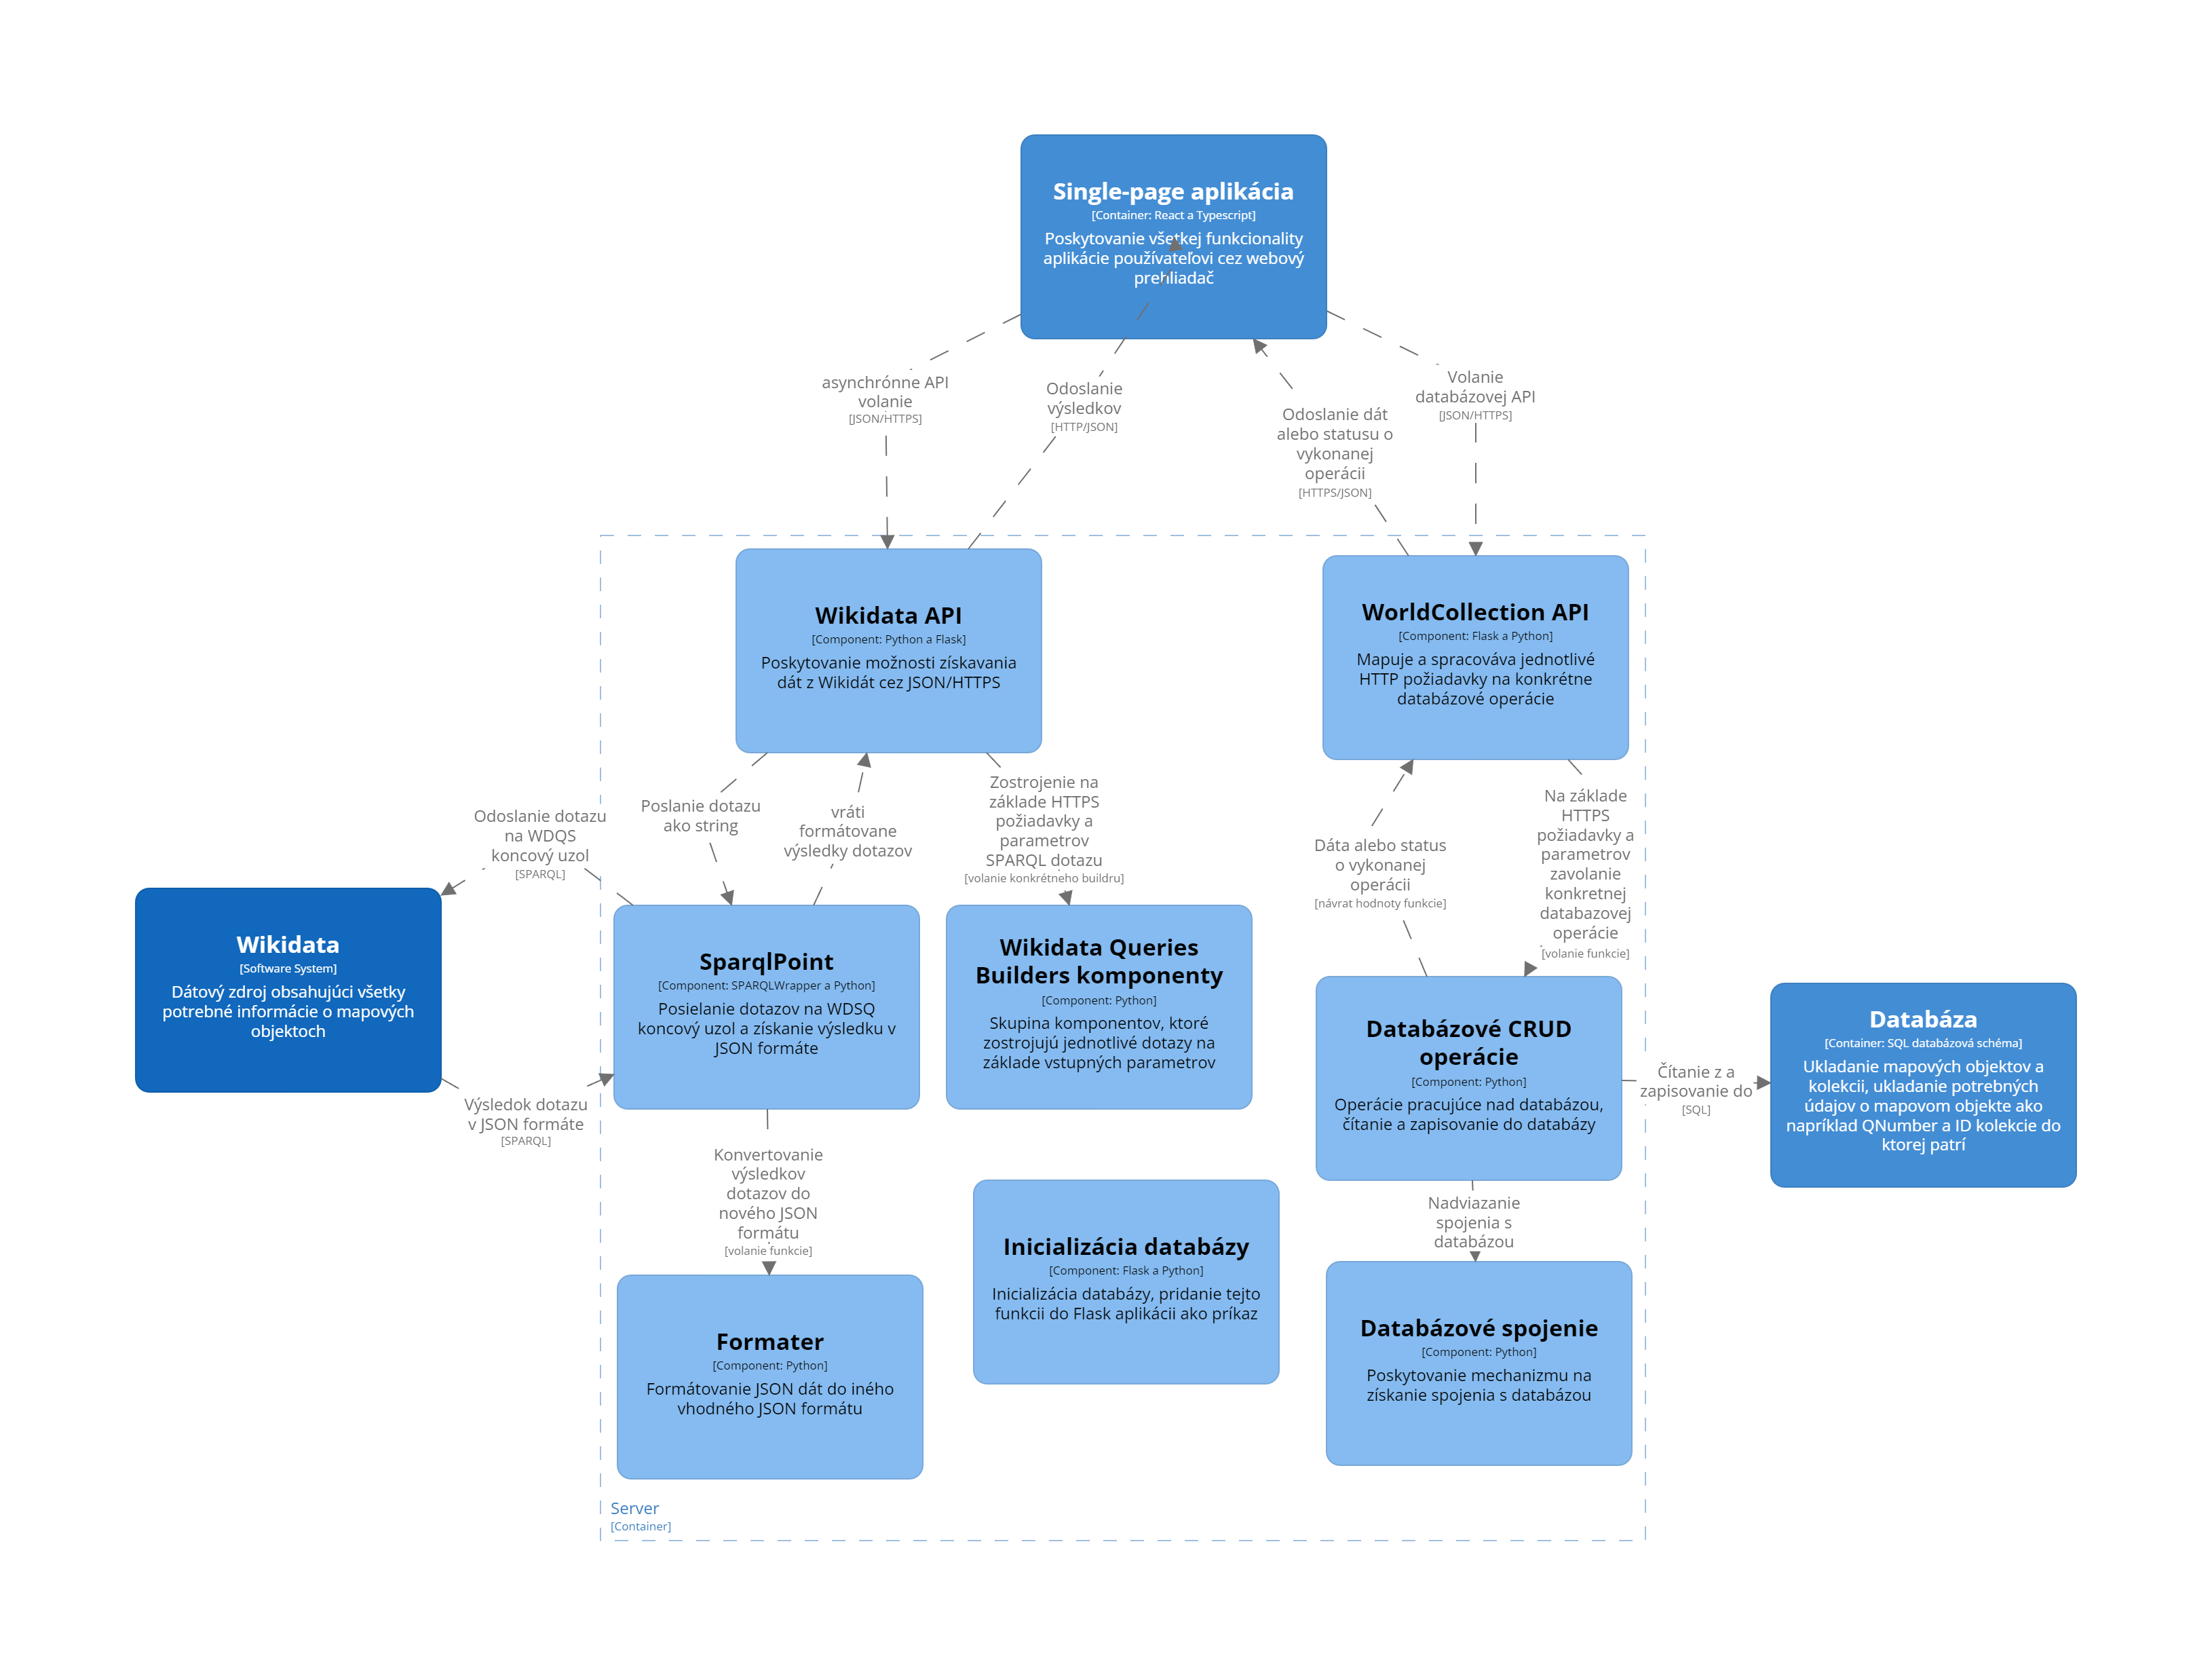
\includegraphics[width=140mm]{../img/structurizr-ServerComponents}
      \caption{Server Komponent diagram }
\end{figure}

Kontajner Server REST API, ktoré je rozdelené do dvoch API. WorldCollectionAPI a WikidataAPI.
Požiadavka príde na server a na zakladá URL Flask technológia
nasmeruje požiadavku na konkrétne koncový uzol, kde sa zavola príslušná funkcia.

WorldCollectionAPI poskytuje rozhranie na čítanie z a zapisovanie do databázy. Na to API využíva databázové CRUD operácie.
Tieto operácie poskytujú všetky potrebné operácie nad databázou, ktoré aplikácia potrebuje využívať.
Každá CRUD operácia reprezentuje základnú operáciu nad databázou ako je napríklad vytvorenie kolekcie, zmenenie názvu kolekcii alebo odstránenie kolekcie.

Pre získanie spojenia s databazou sa použije komponenta Databázové spojenie.

Bokom existuje komponenta Inicializácia databázy. Ta poskytuje mechanizmus vytvorenia a inicializovania databázy na serveri. Tuto funkciu môže využívať iba správca serveru a preto je táto komponenta stojí bokom.
Z toho dôvodu API neposkytuje možnosť zavolať tuto inicializáciu databázy. Tato funkcionalita je pridaná do Aplikácie Flasku ako príkaz, ktorý vie správca serveru zadať do príkazovej riadky.

WikidataAPI sa skladá z funkcii, kde každá funkcia reprezentuje jeden dotaz, ktorý je potrebne poslať na WDQS.
Tieto dotazy je potrebne vytvoriť na základe parametrov. Jedným riešim by bolo napísať pre každú funkciu samostatný
cely dotaz kde stačí len dosadiť vstupné parametre. To by bola ale strašná duplicita a preto navrhneme a implementuje hierarchiu builderov, ktoré
nám skonštruujú dotazy na základe vstupných parametrov. Tuto hierarchiu nám bude reprezentovať komponenta Wikidata Queries Builders.


Všetky tieto buildere vytvoria iba text dotazu. Ten bude následné poskytnutý komponente "SparqlPoint". Tá ma za úlohu poslať dotaz na WDQS a vrátený výsledok vrátiť v Json formáte. Tento výsledok
sa nepošle rovno klientovi. Ešte pred poslaním na SPA bude výsledok skonvertovaný do nového Json formátu, ktorý upravuje Json do podoby aká je vhodná pre našu aplikáciu.

\subsection{ SPA Komponent diagram}

\begin{figure}[h]
      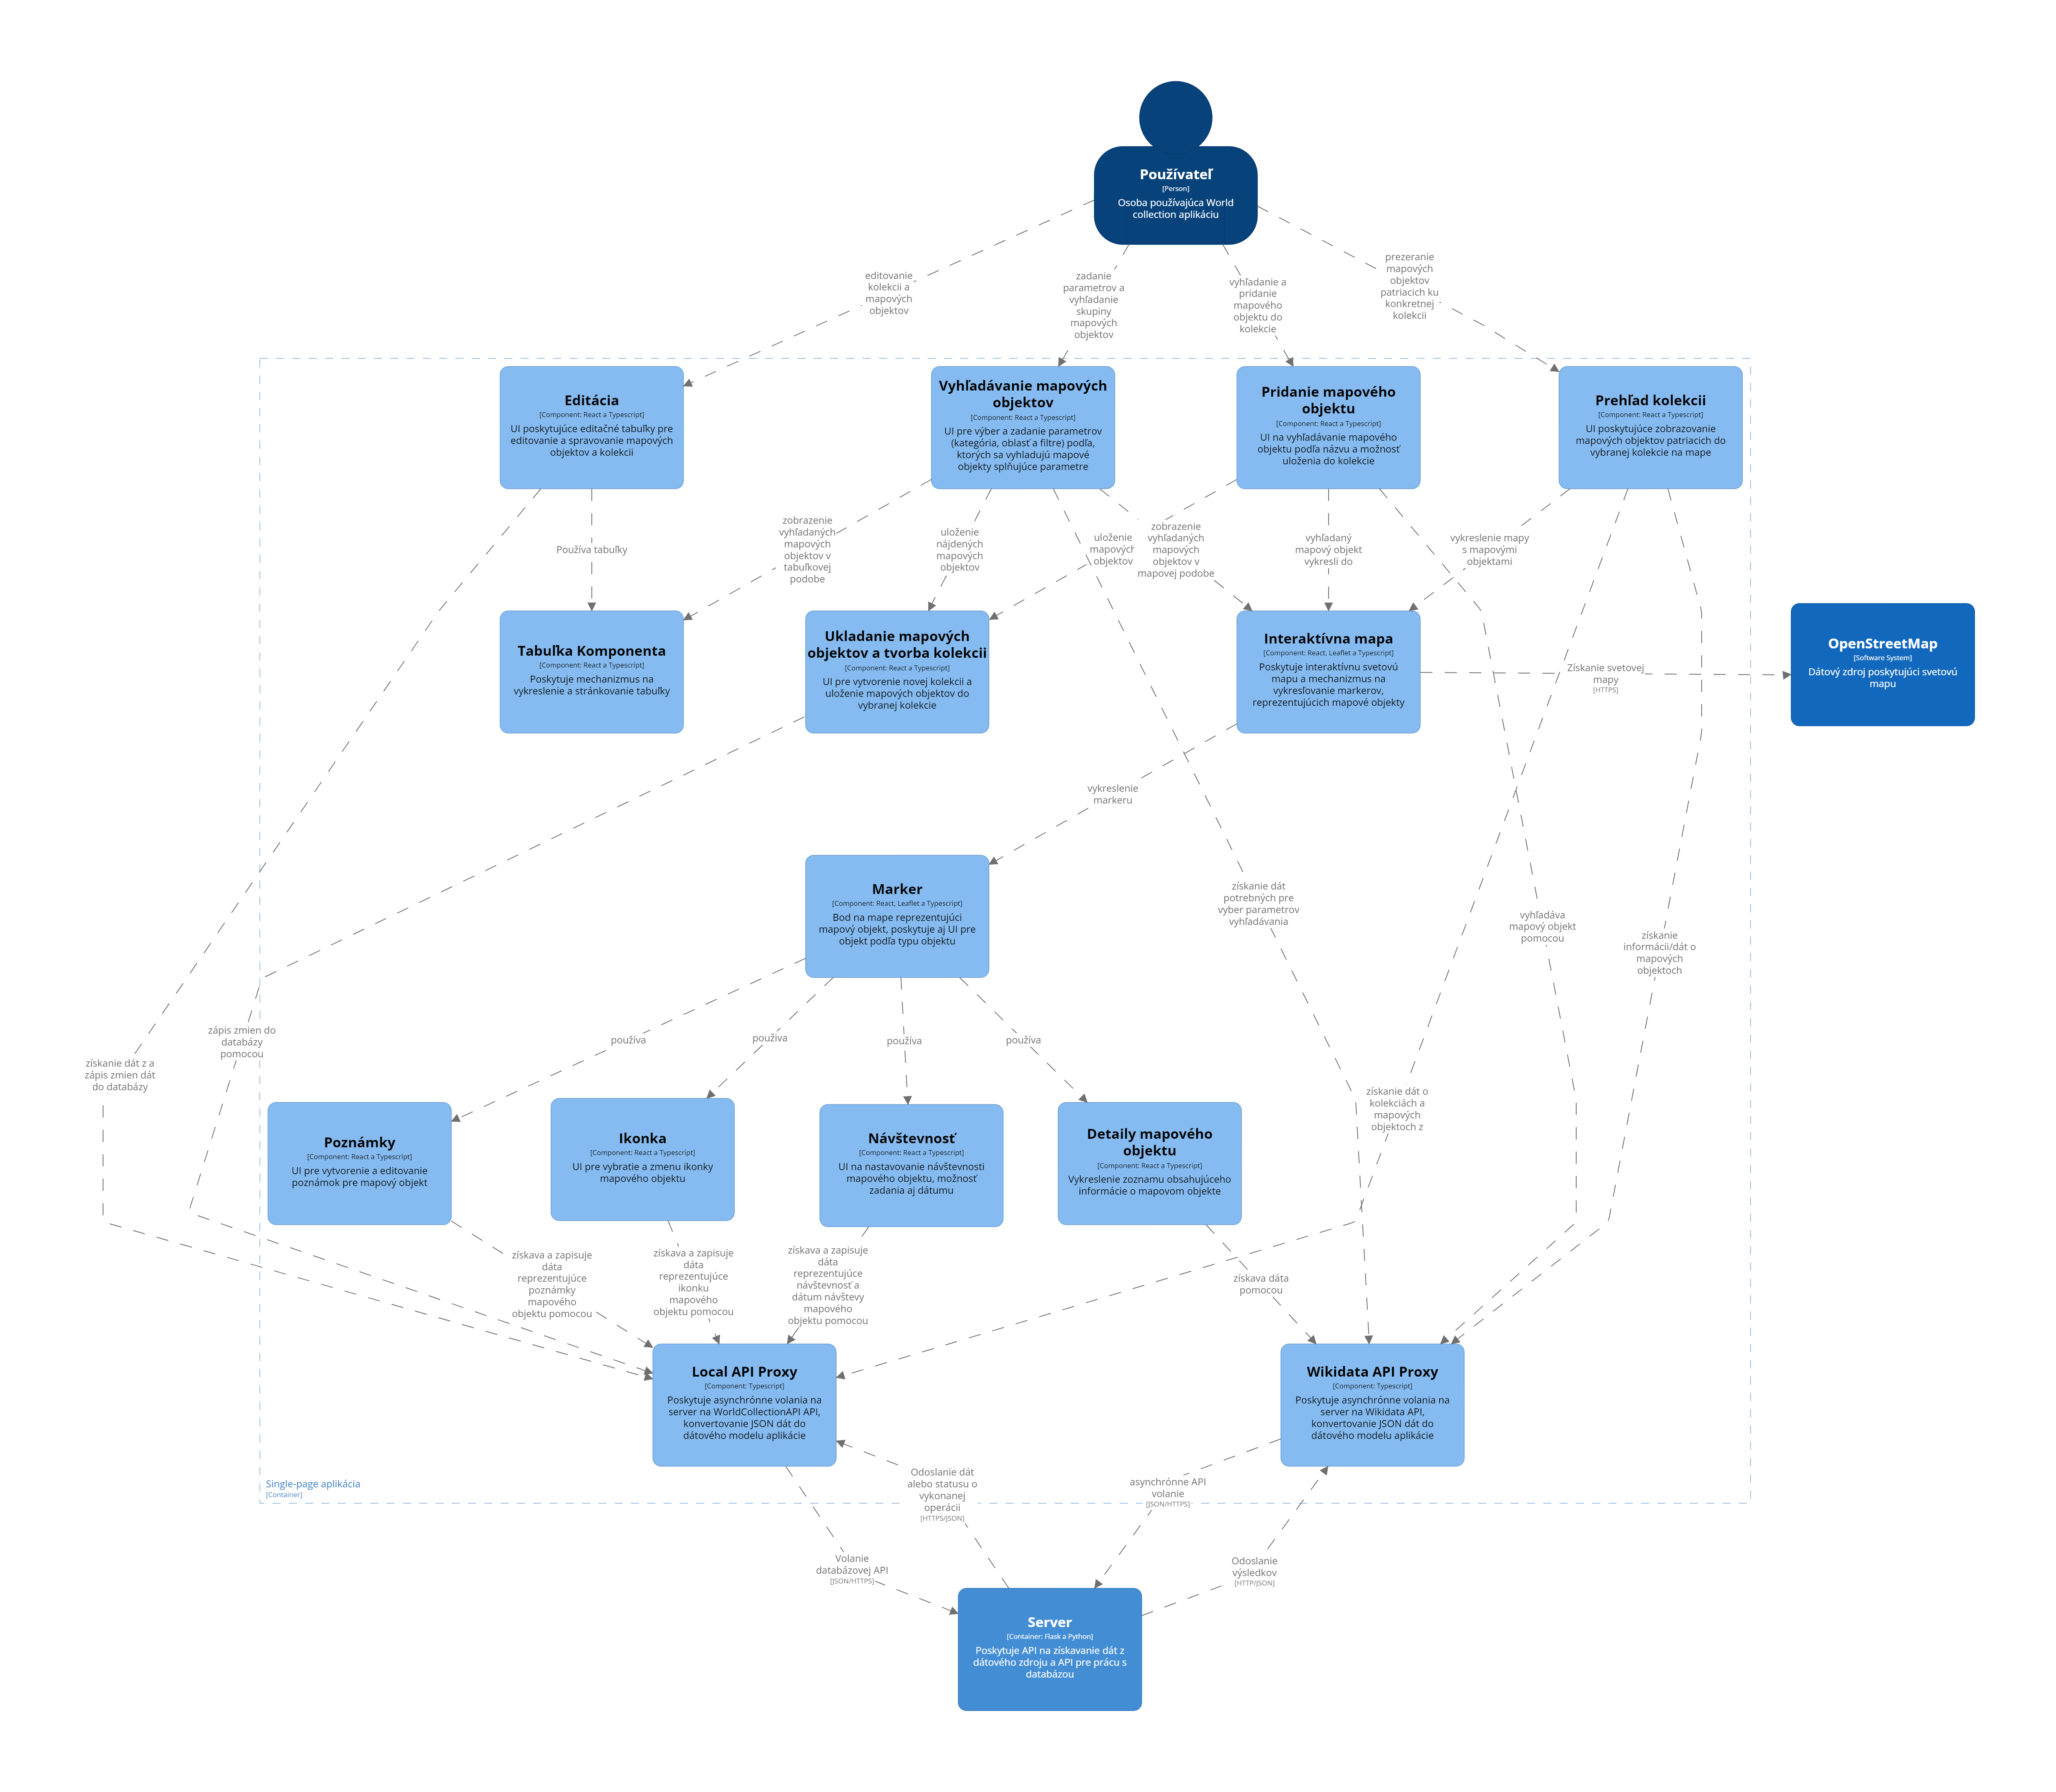
\includegraphics[width=140mm]{../img/structurizr-SinglePageAplicationComponents}
      \caption{ SPA Komponent diagram}
\end{figure}

SPA obsahuje dva APIProxy komponenty. Každá z nich obsahuje funkcie, ktoré robia asynchrónne volania na server pomocou HTTPS požiadavkou.
Parametre sa konvertujú do Json formátu a sú poslane na server v tele požiadavky.

SPA ponúka používateľovi štyri hlavné stavy aplikácie. Medzi jednotlivými stavmi sa používateľ prepína v navigačnom panely.
Tieto stavy sú v modely C4 reprezentované ako komponenty s ktorými používateľ interaguje. Sú to nasledujúce komponenty:

Prehlaď kolekcii - v tomto stave aplikácia zobrazí zoznam kolekcii. Z toho dôvodu musí táto komponenta požiadať Databázovú API o dáta z databázy reprezentujúce kolekcie.
Používateľ je schopný vybrať kolekciu a následne si pozrieť všetky mapové objekty v danej kolekcii. Z toho dôvodu sa zavolá komponenta “Interaktívna mapa”, ktorá poskytuje
interaktívnu mapu. Dáta svetovej mapy sa získavajú pomocou knižnice “Leaflet”. Táto knižnica získava svetovú mapu od poskytovateľa OpenStreetMap.
Do mapy je potrebne vykresliť body (marker) reprezentujúce mapové objekty. Na to slúži komponenta “Marker”, ktorou úlohou je vykresliť bod na mape. Po tom čo používateľ klikne na konkrétny
Bod, aplikácia zobrazí UI okienko kde umožní prezeranie informácii o mapovom objekte (základne informácie, obrázok objektu, možnosť získania detailov, návštevnosť, poznámky),
možnosť napísať poznámky, nastaviť obrázok ikonky bodu alebo uviesť návštevnosť.
Každá z týchto vecí je ako samostatná komponenta. Každá z týchto komponent komunikuje s Databázovou API. pretože je potrebne získavať údaje z databázy alebo vykonané zmeny ako
zmena poznámok, zmena ikonky alebo zmena návštevnosti zapísať do databázy. Výnimkou je komponenta “Detaily mapového objektu”, ktorá poskytuje detaily o objekte a preto je potrebne aby
tieto informácie získala z Wikidat za pomoci “Wikidata API”.

Pridanie mapového objektu - v tomto stave aplikácia zobrazí interaktívnu mapu a možnosť vyhľadať konkrétny mapový objekt. Objekt je vyhľadávaní za pomoci volania “Wikidata API”.
Po tom ako používateľ vyberie nájdený objekt sa na interaktívnej mape zobrazí daný mapový objekt. Preto táto komponenta využíva komponenty “Interantivna mapa” a “Marker”. V tomto konkretnom prípade
Marker nevyužíva všetky štyri komponenty iba “Detaily mapového objektu”. To je z dôvodu, že tento mapový objekt ešte nie je uložený v databáze a preto aplikácia smie poskytnúť iba detaily o mapovom objekte.
Vyhľadané a vybraté mapové objekty aplikácia umožni uložiť do kolekcie. Na to existuje komponenta “Ukladanie mapových objektov a tvorba kolekcii”, ktorá tento mechanizmus zapuzdruje.

Vyhľadanie mapových objektov - v tomto stave aplikácia zobrazí postupne možnosť zadať parametre vyhľadávania. Najprv výber kategórie, následne vyber spôsobu definovania oblasti vyhľadávania, definovanie konkrétnej
oblasti a nakoniec vyber filtrov a zadanie hodnôt daných filtrov. Potom sa uskutoční volanie na “WikidataAPI”, kde sa tieto parametre zabalia do Json formátu a odošlú na server ako náklad v tele požiadavky. Server z nich postaví konkrétny dotaz a pošle ho
na Wikadata. Vrátene výsledky sa zobrazia buď ako tabuľka alebo ako body na interaktívnej mape.

Editácia - v tomto stave aplikácia zobrazí tabuľku s kolekciami a možnosťami dané kolekcie editovať. Každú kolekciu používateľ je schopný otvoriť a následne sa mu
zobrazí editačná tabuľka v ktorej vie editovať mapové objekty v danej kolekcii.
Komponenta získava dáta z komponenty “WorldCollectionAPI API” a vykresľuje tabuľky pomocou komponenty “Tabuľka”, ktorá poskytuje možnosť vykresliť tabuľku s pätičkou tabuľky.
V tejto pätičke vie používateľ sa preklikávať na jednotlivé strany tabuľky, nastavovať počet riadkov na stranu v tabuľke. Po editácii a uložení komponenta urobí API volanie
na server aby boli zmeny uložené v databáze.

\section{Návrh databázy}

V databáze je potrebne mať uložene existujúce kolekcie a aké mapové objekty do kolekcii patria. K mapovému objektu je potrebne udržiavať údaj o jeho QNumber
identifikujúci mapový objekt na Wikidatach pre získavanie informácii o objekte, ale aj iné informácie ako napríklad poznámky alebo dátum návštevnosti.

Pre každú kolekciu si v databáze budeme musieť ukladať dátové informácie ako identifikátor a názov. 
Názov musí byť unikátny. Nemôžeme dovoliť aby v databáze boli uložené dve kolekcie s rovnakým menom.

Pre každý mapový objekt si budeme ukladať nasledujúce informácie:
\begin{itemize}
      \item QNumber objektu
      \item meno mapového objektu
      \item textový reťazec obsahujúci triedy, ktorými je daný objekt inštanciou na Wikidatach.
            Tento udaj by sa dal stále získavať z Wikidat, ale je rozumnejšie si ho raz uložiť a nezaťažovať Wikidata.
            Reťazec obsahuje špeciálny znak, ktorý oddeľuje jednotlivé triedy.
      \item údaj o zemepisnej šírke a výške. Tento udaj by sme mohli získavať cez Wikidata vďaka QNumber, ale je výhodnejšie si tieto informácie uložiť a nezaťažovať neustále Wikidata.
      \item udaj či bol mapový objekt navštívený, pomocou boolean hodnoty
      \item dátum návštevy. Keďže podporujeme možnosť zadať dátum návštevy aj ako rozsah a v rôznych precíznostiach (dátum, mesiac a rok, rok)
            , preto v databáze budeme mat uložene 3 údaje, ktoré spolu budú reprezentovať dátum návštevy. Prvým bude dátum od a druhým dátum do. Tieto
            údaje budú typu Date. Obsahovať budú cely dátum. V prípade zadania dátumu a nie rozsahu bude dátum do prázdnej hodnoty. Tretím údajom bude formát dátumu. V ňom je
            informácie ako reprezentovať dátum návštevy. Čí ako rozsah alebo ako samostatný dátum a v akej precíznosti je potrebne vyjadriť dátum.
      \item názov obrázka ikonky. SPA na strane používateľa na základe názvu tohto udajú zobrazí príslušný obrázok ako ikonku mapového objektu
      \item poznámky ako textový reťazec
\end{itemize}

Zároveň je potrebné si v databáze držať vzťahy medzi kolekciami a mapovými objektami. Vďaka týmto vzťahom budeme schopný povedať do akej kolekcie patri daný mapový objekt. 










